\subsection{Cluster description}\label{sec:viz}

% The last stage of the pipeline is cluster description. 
% This step is fundamental to present the results in the most intelligible and concise format for the end-users to consume it.

% Once we have clusters of data, the next step is to inspect their content to try to grasp their meaning.
% Given the unsupervised learning approach adopted, this interpretation phase is troublesome and time-demanding.

% In order to demonstrate the approach, we report an analysis of FTS data from one full day of operation. %(15/01/2021).

The last stage of the pipeline is cluster description. 
This step is fundamental to present the results in the most intelligible and immediate format for end-users.
Indeed, given the unsupervised learning approach adopted, the interpretation of the clustering output resorts to the manual inspection of each group's content.
This, in turn, potentially mean reading hundreds of error strings, comparing the source and destination information, and spotting suspect time patterns.  
%This implies a troublesome and time-demanding evaluation phase, which partly balances the effort saved by avoiding the collection of a reference dataset of known issues and corresponding solutions.
Therefore, producing a nice and compact visualization of the results is paramount to make the approach effective and avoid excessive manual checks by the operators.
For this reason, the clustering results are summarized into two complementary outputs that are presented to the shifters.

First, the \textit{summary table} represents the most important and informative visualization.
This output is obtained by a first pre-aggregation of the clusters and is organized in a tabular format.
The first three columns provide numeric summaries concerning the  cluster size, the number of unique strings within each cluster, and the corresponding number of unique patterns.
The latter is obtained from the raw strings by means of an \textit{abstraction mechanism} that removes the parametric parts -- like file paths, IP addresses, URLs, checksum values, and so on -- and replaces them by parameter-specific placeholders -- e.g. \textbox{\$FILE\_PATH}, \textbox{\$ADDRESS}, \textbox{\$URL} and  \textbox{\$CHECKSUM}, respectively.
The core part of this visualization is then represented by the \textit{Top 3} section. Here, the three most frequent triplets of \textbox{<pattern>-<source>-<destination>} are reported in descending order for each cluster, alongside their cardinality and the percentage over the cluster size.
Such information provides several precious insights for spotting the source of potential problems, e.g. whether a pattern is responsible for a large number of failures or if it accounts for a conspicuous fraction of the cluster. 
In addition, this representation allows us to investigate the contribution of source/destination pairs to any specific cluster.
In this way, it is possible to discriminate failures based on both the nature of the problem and the location where they occurred.
\Cref{fig:cluster0} shows an example of summary table for the biggest cluster found in the analyzed period.

\begin{landscape}
    \begin{figure}
        \centering
        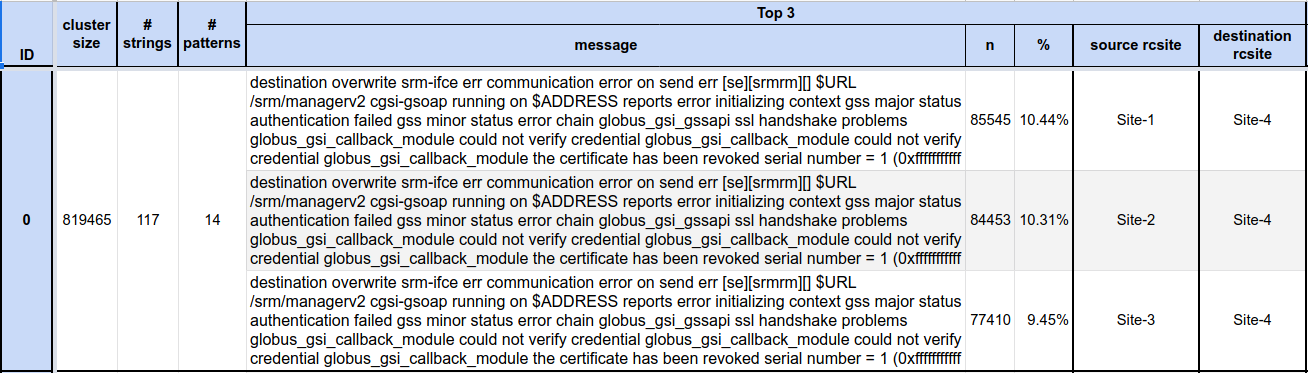
\includegraphics[width=\linewidth]{figures/410_method/cluster0_wide.png}
        \caption{ \textbf{Example cluster summary.}
        The first 3 columns contain numeric summaries of the cluster composition. The \textit{Top-3} section draw a high-level overview of the cluster content summed up by the most frequently observed error triplets of error pattern, source and destination.
        }
        \label{fig:cluster0}
    \end{figure}
\end{landscape}

The second output of the pipeline consists of a time-series chart depicting the temporal evolution of the number of errors generated by each cluster
(\cref{fig:timeplots}).
% (\cref{fig:timeplot_cluster0}).
This piece of information is crucial to discriminate between serious issues that require immediate actions and transient problems. 

Overall, the idea behind our pipeline is to exploit the summary tables and the time plots for each cluster as suggestions of potential issues to investigate further.
In this way, the shifters can have a first grasp of what kind of failures are observed and their corresponding amounts (Top-3 section) and where they are happening (source/destination sites).
Also, by looking at the time charts it is possible to immediately discard transient (\cref{fig:timeplots:transient}) or resolved (\cref{fig:timeplots:resolved}) problems based on the evolution of the number of generated failures over time.


% \begin{figure}
%     \centering
%     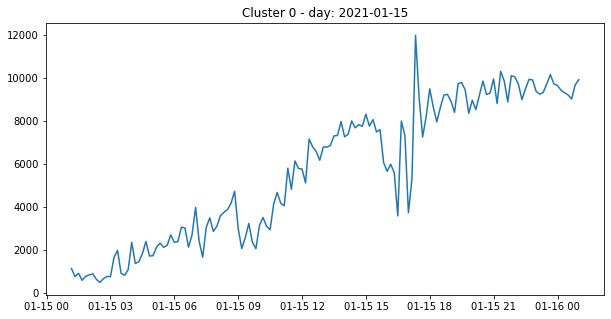
\includegraphics[width=\textwidth]{figures/410_method/timeplot_cluster0.png}
%     \caption{\textbf{Time evolution of cluster 0}. The plot shows the count of errors in bins of 10 minutes.}
%     \label{fig:timeplot_cluster0}
% \end{figure}

\begin{figure}
    \centering
    \subfloat[growing]{
    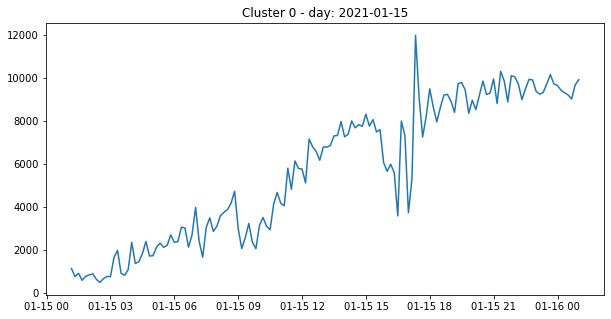
\includegraphics[width=0.5\textwidth]{figures/410_method/timeplot_cluster0.png}
    \label{fig:timeplots:growing}
    }
    \subfloat[transient]{
    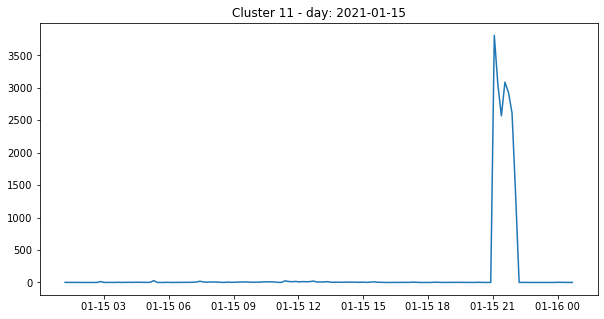
\includegraphics[width=0.5\textwidth]{figures/410_method/timeplots/cluster_11.png}
    \label{fig:timeplots:transient}
    }
    
    \subfloat[resolved]{
    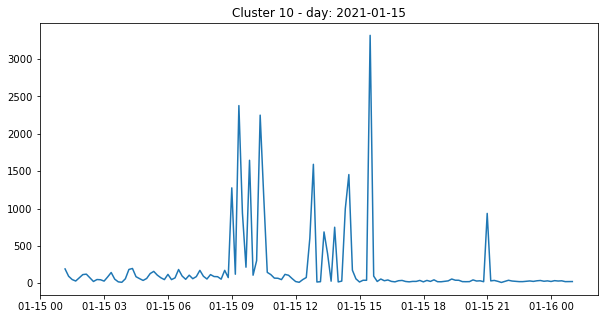
\includegraphics[width=0.5\textwidth]{figures/410_method/timeplots/cluster_10.png}
    \label{fig:timeplots:resolved}
    }
    \subfloat[cyclical]{
    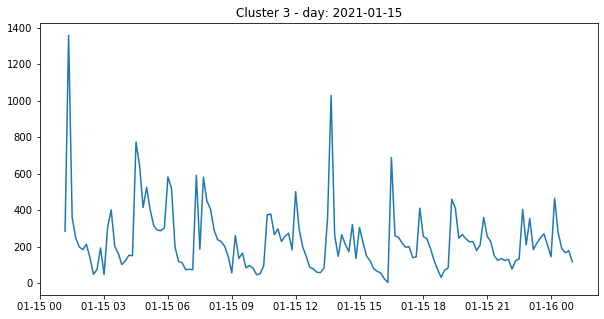
\includegraphics[width=0.5\textwidth]{figures/410_method/timeplots/cluster_3.png}
    \label{fig:timeplots:cyclical}
    }
    \caption{\textbf{Time evolution charts}. The figure illustrates several time patterns for the generated failures in 4 different clusters. Each plot reports the count of errors in bins of 10 minutes.}
    \label{fig:timeplots}
\end{figure}